\documentclass[a4paper,10pt]{article}
\usepackage{tikz}
\usepackage{geometry}
\usepackage{float}
\usetikzlibrary{shapes,positioning,calc,arrows.meta}
\colorlet{lightgray}{gray!30}
\usepackage{xcolor}

\usepackage[pdfusetitle,linkcolor=black,pdfborder={0,0,0}]{hyperref}

\geometry{a4paper,top=1.0in,bottom=1.0in,left=1.0in,right=1.0in}

\author{ \Large Akash Kishore, Akshaya Mohan, Bhavya Jha - 18 5001 \{014,017,035\} }

\date{\Large April 2020}

\title{\Huge \textbf{UCS1412 : Database Lab} \\ \huge \textbf{Student Club Management System}}


%\setkomafont{disposition}{\normalfont\bfseries}

\usepackage{amsmath}
\begin{document}
\maketitle
\hrule
\vspace{10pt}

\section*{ \Large Aim}
\large
\begin{itemize}
	\item Most colleges have a variety of clubs and extra-curricular activities offered to the students. The primary difficulty faced by students is the lack of awareness about these events and activities.
	\item This database management system aims to act as an efficient location and portal for all the information, announcements and events of a college club. 
	\item Club heads can update the events and announcements through this system, and students can also access these details easily.
\end{itemize}

\section*{\Large Functions}
\begin{itemize}
	\item Club heads can add, delete and modify events and add and delete announcements of their respective clubs.
	\item Students can view the information belonging to their clubs.
	\item The number of members and attendees of each event are also recorded.
\end{itemize}

\begin{flushleft}Refer to Figure \ref{fig:diag1} for the design.\end{flushleft}

\section*{Design}
\begin{figure}[H]
\centering
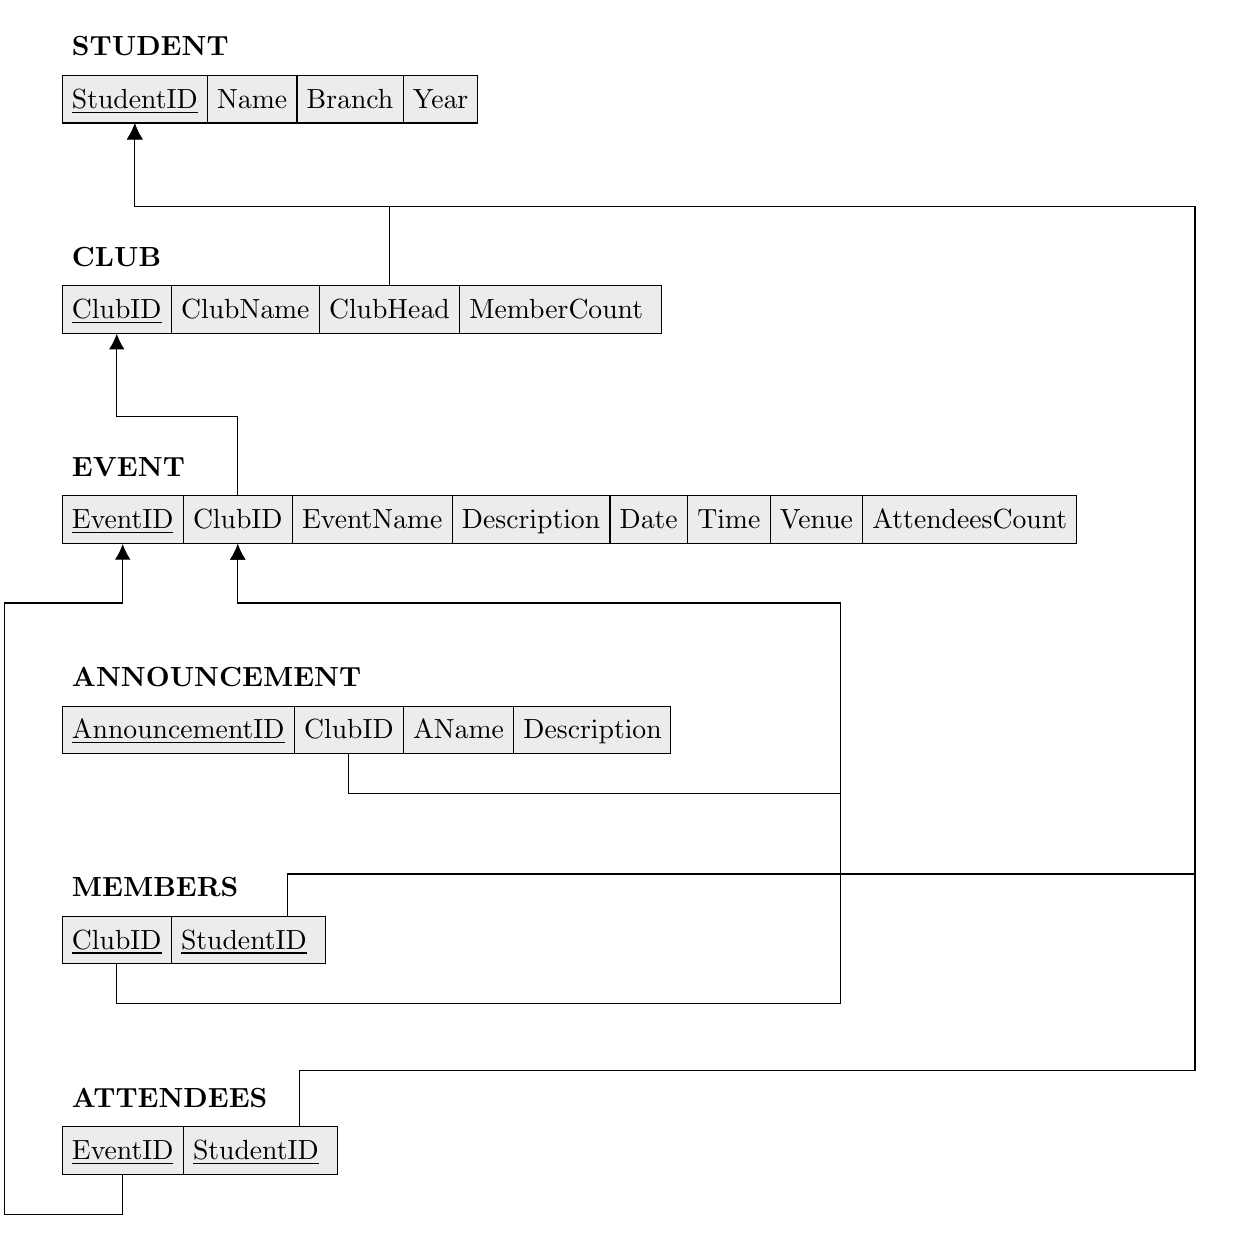
\begin{tikzpicture}[relation/.style={rectangle split, rectangle split parts=#1, rectangle split part align=base, draw, anchor=center, align=center, text height=3mm, text centered}]\hspace*{-0.3cm}

% RELATIONS

\node (studenttitle) {\textbf{STUDENT}};

\node [relation=4, rectangle split horizontal, rectangle split part fill={lightgray!50}, anchor=north west, below=0.67cm of studenttitle.west, anchor=west] (student)
{\underline{StudentID}%
\nodepart{two}   Name
\nodepart{three} Branch
\nodepart{four} Year};

\node [below=2.0cm of student.west, anchor=west] (clubtitle) {\textbf{CLUB}};

\node [relation=4, rectangle split horizontal, rectangle split part fill={lightgray!50}, below=0.67cm of clubtitle.west, anchor=west] (club)
{\underline{ClubID}%
\nodepart{two} ClubName
\nodepart{three} ClubHead
\nodepart{four}  MemberCount };

\node [below=2.0cm of club.west, anchor=west] (eventtitle) {\textbf{EVENT}};

\node [relation=8, rectangle split horizontal, rectangle split part fill={lightgray!50}, anchor=north west, below=0.67cm of eventtitle.west, anchor=west] (event)
{\underline{EventID}%
\nodepart{two}   ClubID
\nodepart{three} EventName
\nodepart{four}  Description
\nodepart{five} Date
\nodepart{six} Time
\nodepart{seven} Venue
\nodepart{eight} AttendeesCount};

\node [below=2.0cm of event.west, anchor=west] (announcementtitle) {\textbf{ANNOUNCEMENT}};

\node [relation=4, rectangle split horizontal, rectangle split part fill={lightgray!50}, anchor=north west, below=0.67cm of announcementtitle.west, anchor=west] (announcement)
{\underline{AnnouncementID}%
\nodepart{two}   ClubID
\nodepart{three} AName
\nodepart{four} Description};

%\node [below=2.0cm of announcement.west, anchor=west] (ell1) {...};

\node [below=2.0cm of announcement.west, anchor=west] (memberstitle) {\textbf{MEMBERS}};

\node [relation=2, rectangle split horizontal, rectangle split part fill={lightgray!50}, anchor=north west, below=0.67cm of memberstitle.west, anchor=west] (members)
{\underline{ClubID} %
\nodepart{two}   \underline{StudentID} };

\node [below=2.0cm of members.west, anchor=west] (attendeestitle) {\textbf{ATTENDEES}};

\node [relation=2, rectangle split horizontal, rectangle split part fill={lightgray!50}, anchor=north west, below=0.67cm of attendeestitle.west, anchor=west] (attendees)
{\underline{EventID}%
\nodepart{two}   \underline{StudentID} };


% FOREIGN KEYS

\draw[-{Latex[length=2mm, width=2mm]}] (club.three north) -- ++(0,1.0) -| (student.one south) ;
%\draw[->] (award.five south) -- ++(0,-0.2) -| ($(award.five south) + (4,0)$) |- ($(student.one south) + (0.25,-0.50)$) -| ($(student.one south) + (0.25,0)$);

\draw[-{Latex[length=2mm, width=2mm]}] (event.two north) -- ++(0,1.0) -| (club.one south);

\draw[-{Latex[length=2mm, width=2mm]}] ($(members.two north) + (0.5,0.0)$) |- ($(event.eight east) + (1.5,-4.5)$) |- ($(club.three north) + (0,1.0)$) -| (student.one south);


\draw[-{Latex[length=2mm, width=2mm]}] (members.one south) -- ++(0,-0.5) -| ($(event.eight east) + (-3.0,-4.0)$) |- ($(event.two south) + (0,-0.75)$) -| (event.two south);


\draw[-{Latex[length=2mm, width=2mm]}] (announcement.two south) -- ++(0,-0.5) -| ($(event.eight east) + (-3.0,-4.0)$) |- ($(event.two south) + (0,-0.75)$) -| (event.two south);


\draw[-{Latex[length=2mm, width=2mm]}] ($(attendees.two north) + (0.5,0.0)$) |- ($(event.eight east) + (1.5,-7.0)$) |- ($(club.three north) + (0,1.0)$) -| (student.one south);

\draw[-{Latex[length=2mm, width=2mm]}] (attendees.one south) -- ++(0,-0.5) -| ($(event.one south) + (-1.5,-0.75)$) -| (event.one south);



\end{tikzpicture}
\caption{Schema Diagram}
\label{fig:diag1}
\end{figure}
\end{document}